\documentclass[1p]{elsarticle_modified}
%\bibliographystyle{elsarticle-num}

%\usepackage[colorlinks]{hyperref}
%\usepackage{abbrmath_seonhwa} %\Abb, \Ascr, \Acal ,\Abf, \Afrak
\usepackage{amsfonts}
\usepackage{amssymb}
\usepackage{amsmath}
\usepackage{amsthm}
\usepackage{scalefnt}
\usepackage{amsbsy}
\usepackage{kotex}
\usepackage{caption}
\usepackage{subfig}
\usepackage{color}
\usepackage{graphicx}
\usepackage{xcolor} %% white, black, red, green, blue, cyan, magenta, yellow
\usepackage{float}
\usepackage{setspace}
\usepackage{hyperref}

\usepackage{tikz}
\usetikzlibrary{arrows}

\usepackage{multirow}
\usepackage{array} % fixed length table
\usepackage{hhline}

%%%%%%%%%%%%%%%%%%%%%
\makeatletter
\renewcommand*\env@matrix[1][\arraystretch]{%
	\edef\arraystretch{#1}%
	\hskip -\arraycolsep
	\let\@ifnextchar\new@ifnextchar
	\array{*\c@MaxMatrixCols c}}
\makeatother %https://tex.stackexchange.com/questions/14071/how-can-i-increase-the-line-spacing-in-a-matrix
%%%%%%%%%%%%%%%

\usepackage[normalem]{ulem}

\newcommand{\msout}[1]{\ifmmode\text{\sout{\ensuremath{#1}}}\else\sout{#1}\fi}
%SOURCE: \msout is \stkout macro in https://tex.stackexchange.com/questions/20609/strikeout-in-math-mode

\newcommand{\cancel}[1]{
	\ifmmode
	{\color{red}\msout{#1}}
	\else
	{\color{red}\sout{#1}}
	\fi
}

\newcommand{\add}[1]{
	{\color{blue}\uwave{#1}}
}

\newcommand{\replace}[2]{
	\ifmmode
	{\color{red}\msout{#1}}{\color{blue}\uwave{#2}}
	\else
	{\color{red}\sout{#1}}{\color{blue}\uwave{#2}}
	\fi
}

\newcommand{\Sol}{\mathcal{S}} %segment
\newcommand{\D}{D} %diagram
\newcommand{\A}{\mathcal{A}} %arc


%%%%%%%%%%%%%%%%%%%%%%%%%%%%%5 test

\def\sl{\operatorname{\textup{SL}}(2,\Cbb)}
\def\psl{\operatorname{\textup{PSL}}(2,\Cbb)}
\def\quan{\mkern 1mu \triangleright \mkern 1mu}

\theoremstyle{definition}
\newtheorem{thm}{Theorem}[section]
\newtheorem{prop}[thm]{Proposition}
\newtheorem{lem}[thm]{Lemma}
\newtheorem{ques}[thm]{Question}
\newtheorem{cor}[thm]{Corollary}
\newtheorem{defn}[thm]{Definition}
\newtheorem{exam}[thm]{Example}
\newtheorem{rmk}[thm]{Remark}
\newtheorem{alg}[thm]{Algorithm}

\newcommand{\I}{\sqrt{-1}}
\begin{document}

%\begin{frontmatter}
%
%\title{Boundary parabolic representations of knots up to 8 crossings}
%
%%% Group authors per affiliation:
%\author{Yunhi Cho} 
%\address{Department of Mathematics, University of Seoul, Seoul, Korea}
%\ead{yhcho@uos.ac.kr}
%
%
%\author{Seonhwa Kim} %\fnref{s_kim}}
%\address{Center for Geometry and Physics, Institute for Basic Science, Pohang, 37673, Korea}
%\ead{ryeona17@ibs.re.kr}
%
%\author{Hyuk Kim}
%\address{Department of Mathematical Sciences, Seoul National University, Seoul 08826, Korea}
%\ead{hyukkim@snu.ac.kr}
%
%\author{Seokbeom Yoon}
%\address{Department of Mathematical Sciences, Seoul National University, Seoul, 08826,  Korea}
%\ead{sbyoon15@snu.ac.kr}
%
%\begin{abstract}
%We find all boundary parabolic representation of knots up to 8 crossings.
%
%\end{abstract}
%\begin{keyword}
%    \MSC[2010] 57M25 
%\end{keyword}
%
%\end{frontmatter}

%\linenumbers
%\tableofcontents
%
\newcommand\colored[1]{\textcolor{white}{\rule[-0.35ex]{0.8em}{1.4ex}}\kern-0.8em\color{red} #1}%
%\newcommand\colored[1]{\textcolor{white}{ #1}\kern-2.17ex	\textcolor{white}{ #1}\kern-1.81ex	\textcolor{white}{ #1}\kern-2.15ex\color{red}#1	}

{\Large $\underline{12a_{1107}~(K12a_{1107})}$}

\setlength{\tabcolsep}{10pt}
\renewcommand{\arraystretch}{1.6}
\vspace{1cm}\begin{tabular}{m{100pt}>{\centering\arraybackslash}m{274pt}}
\multirow{5}{120pt}{
	\centering
	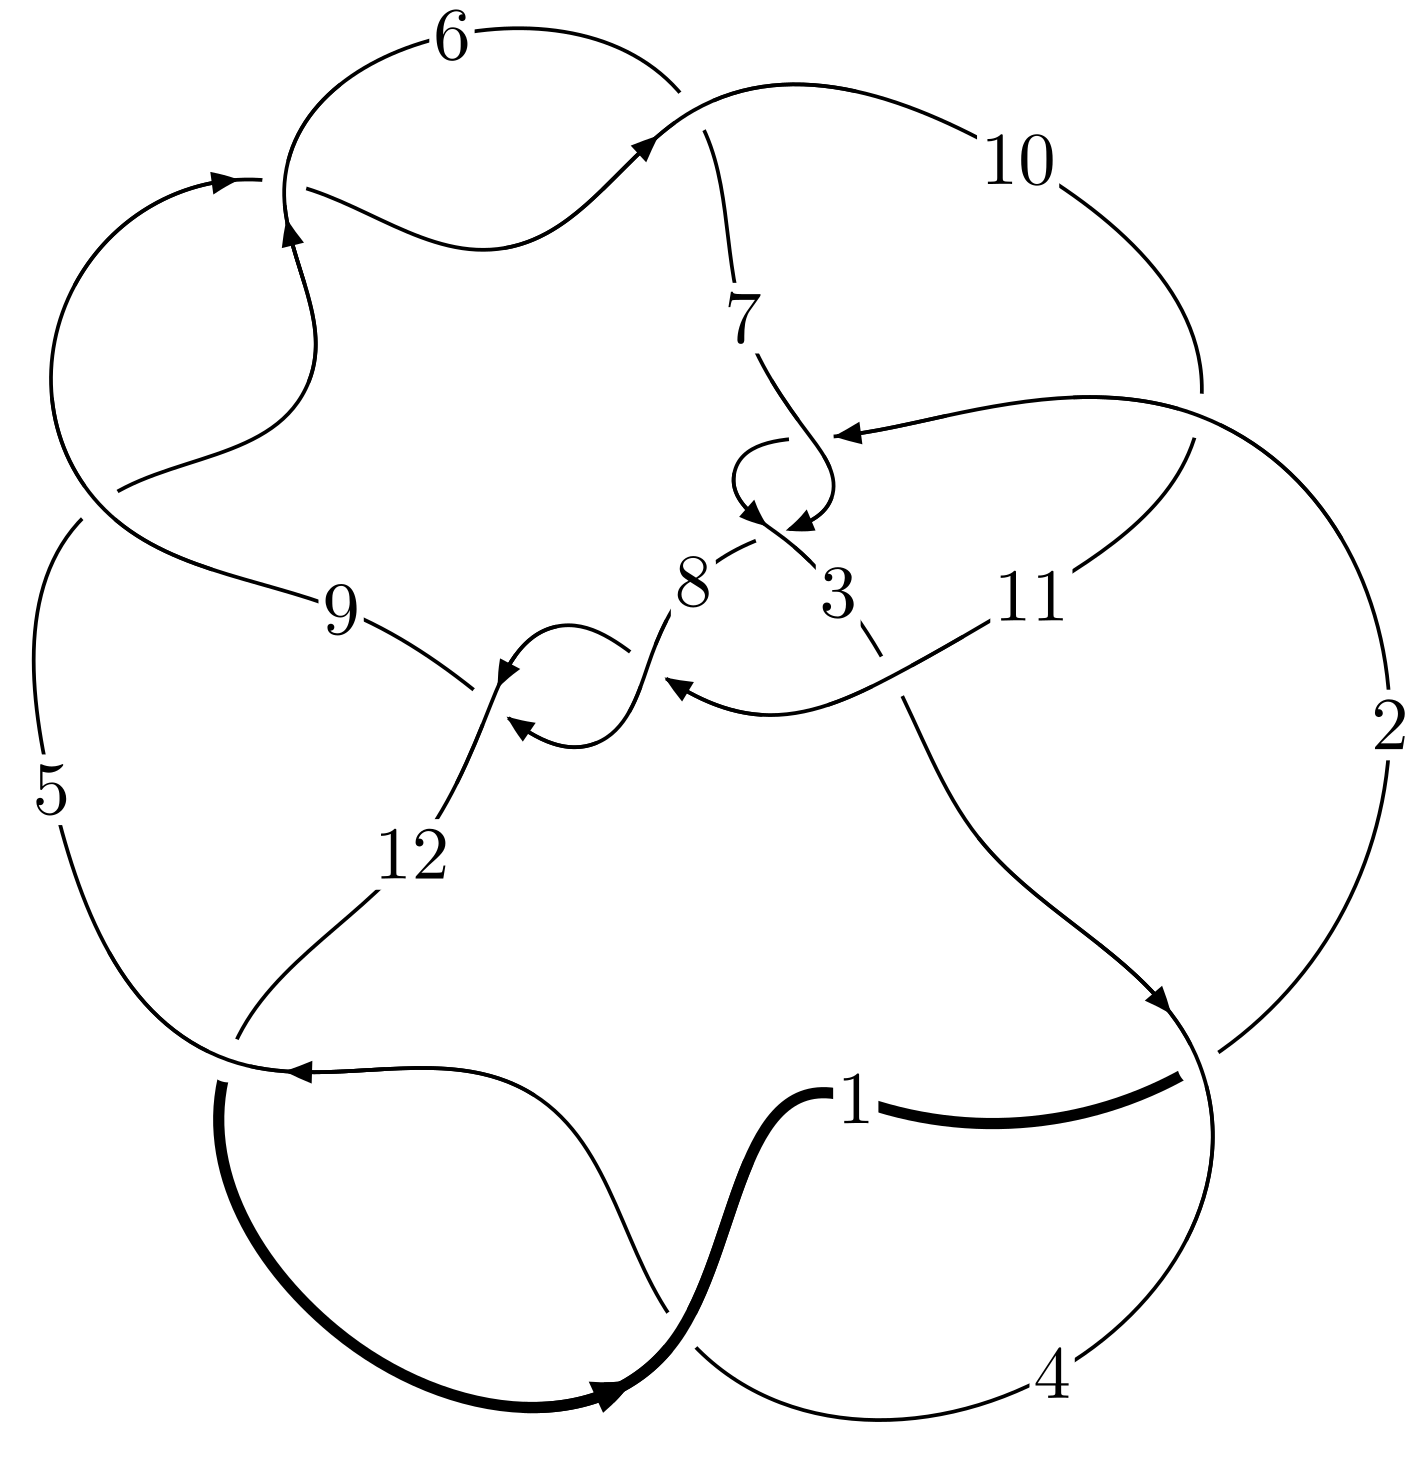
\includegraphics[width=112pt]{../../../GIT/diagram.site/Diagrams/png/1908_12a_1107.png}\\
\ \ \ A knot diagram\footnotemark}&
\allowdisplaybreaks
\textbf{Linearized knot diagam} \\
\cline{2-2}
 &
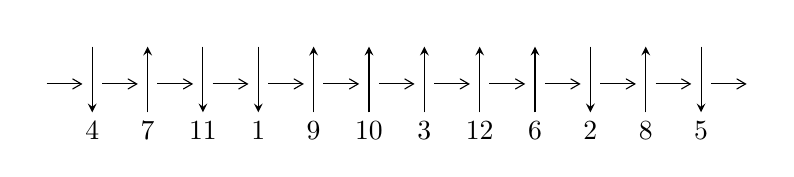
\begin{tikzpicture}[x=20pt, y=17pt]
	% nodes
	\node (C0) at (0, 0) {};
	\node (C1) at (1, 0) {};
	\node (C1U) at (1, +1) {};
	\node (C1D) at (1, -1) {4};

	\node (C2) at (2, 0) {};
	\node (C2U) at (2, +1) {};
	\node (C2D) at (2, -1) {7};

	\node (C3) at (3, 0) {};
	\node (C3U) at (3, +1) {};
	\node (C3D) at (3, -1) {11};

	\node (C4) at (4, 0) {};
	\node (C4U) at (4, +1) {};
	\node (C4D) at (4, -1) {1};

	\node (C5) at (5, 0) {};
	\node (C5U) at (5, +1) {};
	\node (C5D) at (5, -1) {9};

	\node (C6) at (6, 0) {};
	\node (C6U) at (6, +1) {};
	\node (C6D) at (6, -1) {10};

	\node (C7) at (7, 0) {};
	\node (C7U) at (7, +1) {};
	\node (C7D) at (7, -1) {3};

	\node (C8) at (8, 0) {};
	\node (C8U) at (8, +1) {};
	\node (C8D) at (8, -1) {12};

	\node (C9) at (9, 0) {};
	\node (C9U) at (9, +1) {};
	\node (C9D) at (9, -1) {6};

	\node (C10) at (10, 0) {};
	\node (C10U) at (10, +1) {};
	\node (C10D) at (10, -1) {2};

	\node (C11) at (11, 0) {};
	\node (C11U) at (11, +1) {};
	\node (C11D) at (11, -1) {8};

	\node (C12) at (12, 0) {};
	\node (C12U) at (12, +1) {};
	\node (C12D) at (12, -1) {5};
	\node (C13) at (13, 0) {};

	% arrows
	\draw[->,>={angle 60}]
	(C0) edge (C1) (C1) edge (C2) (C2) edge (C3) (C3) edge (C4) (C4) edge (C5) (C5) edge (C6) (C6) edge (C7) (C7) edge (C8) (C8) edge (C9) (C9) edge (C10) (C10) edge (C11) (C11) edge (C12) (C12) edge (C13) ;	\draw[->,>=stealth]
	(C1U) edge (C1D) (C2D) edge (C2U) (C3U) edge (C3D) (C4U) edge (C4D) (C5D) edge (C5U) (C6D) edge (C6U) (C7D) edge (C7U) (C8D) edge (C8U) (C9D) edge (C9U) (C10U) edge (C10D) (C11D) edge (C11U) (C12U) edge (C12D) ;
	\end{tikzpicture} \\
\hhline{~~} \\& 
\textbf{Solving Sequence} \\ \cline{2-2} 
 &
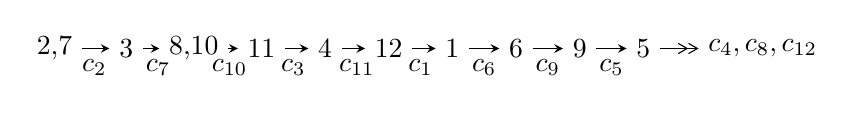
\begin{tikzpicture}[x=23pt, y=7pt]
	% node
	\node (A0) at (-1/8, 0) {2,7};
	\node (A1) at (1, 0) {3};
	\node (A2) at (33/16, 0) {8,10};
	\node (A3) at (25/8, 0) {11};
	\node (A4) at (33/8, 0) {4};
	\node (A5) at (41/8, 0) {12};
	\node (A6) at (49/8, 0) {1};
	\node (A7) at (57/8, 0) {6};
	\node (A8) at (65/8, 0) {9};
	\node (A9) at (73/8, 0) {5};
	\node (C1) at (1/2, -1) {$c_{2}$};
	\node (C2) at (3/2, -1) {$c_{7}$};
	\node (C3) at (21/8, -1) {$c_{10}$};
	\node (C4) at (29/8, -1) {$c_{3}$};
	\node (C5) at (37/8, -1) {$c_{11}$};
	\node (C6) at (45/8, -1) {$c_{1}$};
	\node (C7) at (53/8, -1) {$c_{6}$};
	\node (C8) at (61/8, -1) {$c_{9}$};
	\node (C9) at (69/8, -1) {$c_{5}$};
	\node (A10) at (11, 0) {$c_{4},c_{8},c_{12}$};

	% edge
	\draw[->,>=stealth]	
	(A0) edge (A1) (A1) edge (A2) (A2) edge (A3) (A3) edge (A4) (A4) edge (A5) (A5) edge (A6) (A6) edge (A7) (A7) edge (A8) (A8) edge (A9) ;
	\draw[->>,>={angle 60}]	
	(A9) edge (A10);
\end{tikzpicture} \\ 

\end{tabular} \\

\footnotetext{
The image of knot diagram is generated by the software ``\textbf{Draw programme}" developed by Andrew Bartholomew(\url{http://www.layer8.co.uk/maths/draw/index.htm\#Running-draw}), where we modified some parts for our purpose(\url{https://github.com/CATsTAILs/LinksPainter}).
}\phantom \\ \newline 
\centering \textbf{Ideals for irreducible components\footnotemark of $X_{\text{par}}$} 
 
\begin{align*}
I^u_{1}&=\langle 
1.01048\times10^{165} u^{79}+2.54217\times10^{164} u^{78}+\cdots+3.41950\times10^{164} b-7.77445\times10^{164},\\
\phantom{I^u_{1}}&\phantom{= \langle  }-5.17035\times10^{164} u^{79}+5.54826\times10^{164} u^{78}+\cdots+3.41950\times10^{164} a-3.60849\times10^{163},\\
\phantom{I^u_{1}}&\phantom{= \langle  }u^{80}- u^{79}+\cdots+77 u^2+1\rangle \\
I^u_{2}&=\langle 
232 u^{23}-9371 u^{22}+\cdots+4397 b-14595,\;-13378 u^{23}-29082 u^{22}+\cdots+30779 a-96133,\\
\phantom{I^u_{2}}&\phantom{= \langle  }u^{24}-9 u^{22}+\cdots+2 u-1\rangle \\
\\
\end{align*}
\raggedright * 2 irreducible components of $\dim_{\mathbb{C}}=0$, with total 104 representations.\\
\footnotetext{All coefficients of polynomials are rational numbers. But the coefficients are sometimes approximated in decimal forms when there is not enough margin.}
\newpage
\renewcommand{\arraystretch}{1}
\centering \section*{I. $I^u_{1}= \langle 1.01\times10^{165} u^{79}+2.54\times10^{164} u^{78}+\cdots+3.42\times10^{164} b-7.77\times10^{164},\;-5.17\times10^{164} u^{79}+5.55\times10^{164} u^{78}+\cdots+3.42\times10^{164} a-3.61\times10^{163},\;u^{80}- u^{79}+\cdots+77 u^2+1 \rangle$}
\flushleft \textbf{(i) Arc colorings}\\
\begin{tabular}{m{7pt} m{180pt} m{7pt} m{180pt} }
\flushright $a_{2}=$&$\begin{pmatrix}1\\0\end{pmatrix}$ \\
\flushright $a_{7}=$&$\begin{pmatrix}0\\u\end{pmatrix}$ \\
\flushright $a_{3}=$&$\begin{pmatrix}1\\- u^2\end{pmatrix}$ \\
\flushright $a_{8}=$&$\begin{pmatrix}u\\- u^3+u\end{pmatrix}$ \\
\flushright $a_{10}=$&$\begin{pmatrix}1.51202 u^{79}-1.62254 u^{78}+\cdots+113.235 u+0.105527\\-2.95505 u^{79}-0.743435 u^{78}+\cdots+11.1242 u+2.27356\end{pmatrix}$ \\
\flushright $a_{11}=$&$\begin{pmatrix}4.46707 u^{79}-0.879103 u^{78}+\cdots+102.111 u-2.16804\\-2.95505 u^{79}-0.743435 u^{78}+\cdots+11.1242 u+2.27356\end{pmatrix}$ \\
\flushright $a_{4}=$&$\begin{pmatrix}1.67385 u^{79}+0.289420 u^{78}+\cdots-1.17646 u-12.9982\\-1.18420 u^{79}-0.192329 u^{78}+\cdots+0.413449 u+1.05286\end{pmatrix}$ \\
\flushright $a_{12}=$&$\begin{pmatrix}2.40314 u^{79}-1.41293 u^{78}+\cdots+104.976 u-0.569502\\-1.63115 u^{79}-0.400807 u^{78}+\cdots+11.9253 u+1.27435\end{pmatrix}$ \\
\flushright $a_{1}=$&$\begin{pmatrix}-2.08629 u^{79}-0.293098 u^{78}+\cdots+0.912283 u+1.62816\\-0.844189 u^{79}-0.0173289 u^{78}+\cdots-1.90524 u+1.58429\end{pmatrix}$ \\
\flushright $a_{6}=$&$\begin{pmatrix}3.48631 u^{79}-2.36607 u^{78}+\cdots+164.350 u-0.593819\\3.21212 u^{79}+0.854157 u^{78}+\cdots+14.2195 u-2.45641\end{pmatrix}$ \\
\flushright $a_{9}=$&$\begin{pmatrix}-0.580067 u^{79}+3.15254 u^{78}+\cdots-124.634 u-1.51358\\0.746830 u^{79}+0.320814 u^{78}+\cdots-17.3276 u-0.655648\end{pmatrix}$ \\
\flushright $a_{5}=$&$\begin{pmatrix}-3.47372 u^{79}+0.944591 u^{78}+\cdots-3.30266 u+1.85928\\1.80989 u^{79}+0.553280 u^{78}+\cdots-12.0166 u-1.68220\end{pmatrix}$\\&\end{tabular}
\flushleft \textbf{(ii) Obstruction class $= -1$}\\~\\
\flushleft \textbf{(iii) Cusp Shapes $= -5.07525 u^{79}-1.43220 u^{78}+\cdots-10.6961 u+15.3492$}\\~\\
\newpage\renewcommand{\arraystretch}{1}
\flushleft \textbf{(iv) u-Polynomials at the component}\newline \\
\begin{tabular}{m{50pt}|m{274pt}}
Crossings & \hspace{64pt}u-Polynomials at each crossing \\
\hline $$\begin{aligned}c_{1},c_{4},c_{12}\end{aligned}$$&$\begin{aligned}
&u^{80}-3 u^{79}+\cdots+934 u-73
\end{aligned}$\\
\hline $$\begin{aligned}c_{2},c_{7}\end{aligned}$$&$\begin{aligned}
&u^{80}+u^{79}+\cdots+77 u^2+1
\end{aligned}$\\
\hline $$\begin{aligned}c_{3}\end{aligned}$$&$\begin{aligned}
&u^{80}-2 u^{79}+\cdots+237896 u-72979
\end{aligned}$\\
\hline $$\begin{aligned}c_{5},c_{6},c_{9}\end{aligned}$$&$\begin{aligned}
&u^{80}-4 u^{79}+\cdots-2139 u-529
\end{aligned}$\\
\hline $$\begin{aligned}c_{8},c_{11}\end{aligned}$$&$\begin{aligned}
&u^{80}-43 u^{78}+\cdots+2193 u+583
\end{aligned}$\\
\hline $$\begin{aligned}c_{10}\end{aligned}$$&$\begin{aligned}
&u^{80}+6 u^{79}+\cdots+1524620 u-140713
\end{aligned}$\\
\hline
\end{tabular}\\~\\
\newpage\renewcommand{\arraystretch}{1}
\flushleft \textbf{(v) Riley Polynomials at the component}\newline \\
\begin{tabular}{m{50pt}|m{274pt}}
Crossings & \hspace{64pt}Riley Polynomials at each crossing \\
\hline $$\begin{aligned}c_{1},c_{4},c_{12}\end{aligned}$$&$\begin{aligned}
&y^{80}+93 y^{79}+\cdots-288502 y+5329
\end{aligned}$\\
\hline $$\begin{aligned}c_{2},c_{7}\end{aligned}$$&$\begin{aligned}
&y^{80}-65 y^{79}+\cdots+154 y+1
\end{aligned}$\\
\hline $$\begin{aligned}c_{3}\end{aligned}$$&$\begin{aligned}
&y^{80}+42 y^{79}+\cdots+54740796004 y+5325934441
\end{aligned}$\\
\hline $$\begin{aligned}c_{5},c_{6},c_{9}\end{aligned}$$&$\begin{aligned}
&y^{80}-96 y^{79}+\cdots-7161073 y+279841
\end{aligned}$\\
\hline $$\begin{aligned}c_{8},c_{11}\end{aligned}$$&$\begin{aligned}
&y^{80}-86 y^{79}+\cdots+12819505 y+339889
\end{aligned}$\\
\hline $$\begin{aligned}c_{10}\end{aligned}$$&$\begin{aligned}
&y^{80}+46 y^{79}+\cdots-642253205014 y+19800148369
\end{aligned}$\\
\hline
\end{tabular}\\~\\
\newpage\flushleft \textbf{(vi) Complex Volumes and Cusp Shapes}
$$\begin{array}{c|c|c}  
\text{Solutions to }I^u_{1}& \I (\text{vol} + \sqrt{-1}CS) & \text{Cusp shape}\\
 \hline 
\begin{aligned}
u &= \phantom{-}0.696936 + 0.729645 I \\
a &= \phantom{-}0.632882 - 0.912130 I \\
b &= \phantom{-}0.021106 - 0.373710 I\end{aligned}
 & \phantom{-}4.15739 + 0.27185 I & \phantom{-0.000000 } 0 \\ \hline\begin{aligned}
u &= \phantom{-}0.696936 - 0.729645 I \\
a &= \phantom{-}0.632882 + 0.912130 I \\
b &= \phantom{-}0.021106 + 0.373710 I\end{aligned}
 & \phantom{-}4.15739 - 0.27185 I & \phantom{-0.000000 } 0 \\ \hline\begin{aligned}
u &= \phantom{-}0.135002 + 0.952540 I \\
a &= \phantom{-}0.864710 - 0.639597 I \\
b &= \phantom{-}0.728429 - 0.940911 I\end{aligned}
 & \phantom{-}9.53387 + 5.61294 I & \phantom{-0.000000 } 0 \\ \hline\begin{aligned}
u &= \phantom{-}0.135002 - 0.952540 I \\
a &= \phantom{-}0.864710 + 0.639597 I \\
b &= \phantom{-}0.728429 + 0.940911 I\end{aligned}
 & \phantom{-}9.53387 - 5.61294 I & \phantom{-0.000000 } 0 \\ \hline\begin{aligned}
u &= \phantom{-}0.868294 + 0.372933 I \\
a &= -1.101470 + 0.485003 I \\
b &= -0.868224 + 0.272648 I\end{aligned}
 & \phantom{-}4.75188 + 3.71337 I & \phantom{-0.000000 } 0 \\ \hline\begin{aligned}
u &= \phantom{-}0.868294 - 0.372933 I \\
a &= -1.101470 - 0.485003 I \\
b &= -0.868224 - 0.272648 I\end{aligned}
 & \phantom{-}4.75188 - 3.71337 I & \phantom{-0.000000 } 0 \\ \hline\begin{aligned}
u &= \phantom{-}0.040864 + 0.925223 I \\
a &= \phantom{-}0.07581 - 1.48298 I \\
b &= \phantom{-}0.241815 - 0.985617 I\end{aligned}
 & \phantom{-}3.95442 + 1.49798 I & \phantom{-0.000000 } 0 \\ \hline\begin{aligned}
u &= \phantom{-}0.040864 - 0.925223 I \\
a &= \phantom{-}0.07581 + 1.48298 I \\
b &= \phantom{-}0.241815 + 0.985617 I\end{aligned}
 & \phantom{-}3.95442 - 1.49798 I & \phantom{-0.000000 } 0 \\ \hline\begin{aligned}
u &= -0.588597 + 0.700636 I \\
a &= -0.397248 + 0.207196 I \\
b &= -0.543099 - 0.075426 I\end{aligned}
 & \phantom{-}1.06681 - 2.17703 I & \phantom{-0.000000 } 0 \\ \hline\begin{aligned}
u &= -0.588597 - 0.700636 I \\
a &= -0.397248 - 0.207196 I \\
b &= -0.543099 + 0.075426 I\end{aligned}
 & \phantom{-}1.06681 + 2.17703 I & \phantom{-0.000000 } 0\\
 \hline 
 \end{array}$$\newpage$$\begin{array}{c|c|c}  
\text{Solutions to }I^u_{1}& \I (\text{vol} + \sqrt{-1}CS) & \text{Cusp shape}\\
 \hline 
\begin{aligned}
u &= -0.142022 + 1.091210 I \\
a &= -0.315318 - 0.470004 I \\
b &= -0.290486 - 0.637626 I\end{aligned}
 & \phantom{-}1.73943 - 2.57033 I & \phantom{-0.000000 } 0 \\ \hline\begin{aligned}
u &= -0.142022 - 1.091210 I \\
a &= -0.315318 + 0.470004 I \\
b &= -0.290486 + 0.637626 I\end{aligned}
 & \phantom{-}1.73943 + 2.57033 I & \phantom{-0.000000 } 0 \\ \hline\begin{aligned}
u &= -1.126310 + 0.089569 I \\
a &= -0.442007 + 0.484742 I \\
b &= -0.071623 - 0.866787 I\end{aligned}
 & \phantom{-}2.07180 - 0.39101 I & \phantom{-0.000000 } 0 \\ \hline\begin{aligned}
u &= -1.126310 - 0.089569 I \\
a &= -0.442007 - 0.484742 I \\
b &= -0.071623 + 0.866787 I\end{aligned}
 & \phantom{-}2.07180 + 0.39101 I & \phantom{-0.000000 } 0 \\ \hline\begin{aligned}
u &= \phantom{-}0.010153 + 0.860616 I \\
a &= \phantom{-}0.00315 - 1.86109 I \\
b &= -0.523475 - 1.293000 I\end{aligned}
 & \phantom{-}11.67760 - 3.21420 I & \phantom{-}7.86067 + 0. I\phantom{ +0.000000I} \\ \hline\begin{aligned}
u &= \phantom{-}0.010153 - 0.860616 I \\
a &= \phantom{-}0.00315 + 1.86109 I \\
b &= -0.523475 + 1.293000 I\end{aligned}
 & \phantom{-}11.67760 + 3.21420 I & \phantom{-}7.86067 + 0. I\phantom{ +0.000000I} \\ \hline\begin{aligned}
u &= \phantom{-}1.176850 + 0.214087 I \\
a &= \phantom{-}0.453143 + 0.396474 I \\
b &= \phantom{-}0.521520 - 1.178590 I\end{aligned}
 & \phantom{-}2.04646 + 3.46770 I & \phantom{-0.000000 } 0 \\ \hline\begin{aligned}
u &= \phantom{-}1.176850 - 0.214087 I \\
a &= \phantom{-}0.453143 - 0.396474 I \\
b &= \phantom{-}0.521520 + 1.178590 I\end{aligned}
 & \phantom{-}2.04646 - 3.46770 I & \phantom{-0.000000 } 0 \\ \hline\begin{aligned}
u &= -0.785016\phantom{ +0.000000I} \\
a &= \phantom{-}1.33024\phantom{ +0.000000I} \\
b &= \phantom{-}1.08366\phantom{ +0.000000I}\end{aligned}
 & \phantom{-}1.13184\phantom{ +0.000000I} & \phantom{-}8.48010\phantom{ +0.000000I} \\ \hline\begin{aligned}
u &= \phantom{-}1.222590 + 0.169019 I \\
a &= -0.366542 + 0.187924 I \\
b &= -0.813785 - 1.003570 I\end{aligned}
 & \phantom{-}5.24817 + 2.02818 I & \phantom{-0.000000 } 0\\
 \hline 
 \end{array}$$\newpage$$\begin{array}{c|c|c}  
\text{Solutions to }I^u_{1}& \I (\text{vol} + \sqrt{-1}CS) & \text{Cusp shape}\\
 \hline 
\begin{aligned}
u &= \phantom{-}1.222590 - 0.169019 I \\
a &= -0.366542 - 0.187924 I \\
b &= -0.813785 + 1.003570 I\end{aligned}
 & \phantom{-}5.24817 - 2.02818 I & \phantom{-0.000000 } 0 \\ \hline\begin{aligned}
u &= \phantom{-}1.243590 + 0.025750 I \\
a &= \phantom{-}0.491354 + 0.508234 I \\
b &= -0.299282 - 1.114900 I\end{aligned}
 & \phantom{-}7.67920 - 1.91271 I & \phantom{-0.000000 } 0 \\ \hline\begin{aligned}
u &= \phantom{-}1.243590 - 0.025750 I \\
a &= \phantom{-}0.491354 - 0.508234 I \\
b &= -0.299282 + 1.114900 I\end{aligned}
 & \phantom{-}7.67920 + 1.91271 I & \phantom{-0.000000 } 0 \\ \hline\begin{aligned}
u &= -1.233740 + 0.160122 I \\
a &= \phantom{-}0.416652 - 0.189134 I \\
b &= \phantom{-}1.68403 - 1.29569 I\end{aligned}
 & \phantom{-}12.34390 - 2.02934 I & \phantom{-0.000000 } 0 \\ \hline\begin{aligned}
u &= -1.233740 - 0.160122 I \\
a &= \phantom{-}0.416652 + 0.189134 I \\
b &= \phantom{-}1.68403 + 1.29569 I\end{aligned}
 & \phantom{-}12.34390 + 2.02934 I & \phantom{-0.000000 } 0 \\ \hline\begin{aligned}
u &= -0.224335 + 1.251370 I \\
a &= \phantom{-}0.396579 + 1.240710 I \\
b &= \phantom{-}0.439295 + 1.205560 I\end{aligned}
 & \phantom{-}17.5268 - 9.1987 I & \phantom{-0.000000 } 0 \\ \hline\begin{aligned}
u &= -0.224335 - 1.251370 I \\
a &= \phantom{-}0.396579 - 1.240710 I \\
b &= \phantom{-}0.439295 - 1.205560 I\end{aligned}
 & \phantom{-}17.5268 + 9.1987 I & \phantom{-0.000000 } 0 \\ \hline\begin{aligned}
u &= -1.253320 + 0.226787 I \\
a &= -0.545170 + 0.251974 I \\
b &= -0.76985 - 1.68601 I\end{aligned}
 & \phantom{-}7.94638 - 5.57424 I & \phantom{-0.000000 } 0 \\ \hline\begin{aligned}
u &= -1.253320 - 0.226787 I \\
a &= -0.545170 - 0.251974 I \\
b &= -0.76985 + 1.68601 I\end{aligned}
 & \phantom{-}7.94638 + 5.57424 I & \phantom{-0.000000 } 0 \\ \hline\begin{aligned}
u &= \phantom{-}1.276730 + 0.036383 I \\
a &= \phantom{-}1.228410 - 0.105767 I \\
b &= \phantom{-}2.64332 - 1.67262 I\end{aligned}
 & \phantom{-}19.4910 - 3.4464 I & \phantom{-0.000000 } 0\\
 \hline 
 \end{array}$$\newpage$$\begin{array}{c|c|c}  
\text{Solutions to }I^u_{1}& \I (\text{vol} + \sqrt{-1}CS) & \text{Cusp shape}\\
 \hline 
\begin{aligned}
u &= \phantom{-}1.276730 - 0.036383 I \\
a &= \phantom{-}1.228410 + 0.105767 I \\
b &= \phantom{-}2.64332 + 1.67262 I\end{aligned}
 & \phantom{-}19.4910 + 3.4464 I & \phantom{-0.000000 } 0 \\ \hline\begin{aligned}
u &= -1.265650 + 0.190509 I \\
a &= \phantom{-}0.244681 + 0.771958 I \\
b &= \phantom{-}0.017983 - 0.909709 I\end{aligned}
 & \phantom{-}5.35611 - 2.38954 I & \phantom{-0.000000 } 0 \\ \hline\begin{aligned}
u &= -1.265650 - 0.190509 I \\
a &= \phantom{-}0.244681 - 0.771958 I \\
b &= \phantom{-}0.017983 + 0.909709 I\end{aligned}
 & \phantom{-}5.35611 + 2.38954 I & \phantom{-0.000000 } 0 \\ \hline\begin{aligned}
u &= -1.299340 + 0.029424 I \\
a &= -1.217230 + 0.003891 I \\
b &= -1.83036 - 1.15663 I\end{aligned}
 & \phantom{-}12.50960 + 1.28371 I & \phantom{-0.000000 } 0 \\ \hline\begin{aligned}
u &= -1.299340 - 0.029424 I \\
a &= -1.217230 - 0.003891 I \\
b &= -1.83036 + 1.15663 I\end{aligned}
 & \phantom{-}12.50960 - 1.28371 I & \phantom{-0.000000 } 0 \\ \hline\begin{aligned}
u &= \phantom{-}1.299070 + 0.193597 I \\
a &= -0.237125 + 1.091620 I \\
b &= \phantom{-}0.267604 - 0.949221 I\end{aligned}
 & \phantom{-}12.85860 + 2.75004 I & \phantom{-0.000000 } 0 \\ \hline\begin{aligned}
u &= \phantom{-}1.299070 - 0.193597 I \\
a &= -0.237125 - 1.091620 I \\
b &= \phantom{-}0.267604 + 0.949221 I\end{aligned}
 & \phantom{-}12.85860 - 2.75004 I & \phantom{-0.000000 } 0 \\ \hline\begin{aligned}
u &= \phantom{-}1.326140 + 0.028464 I \\
a &= \phantom{-}1.269620 + 0.151823 I \\
b &= \phantom{-}0.866280 - 0.943954 I\end{aligned}
 & \phantom{-}12.89430 + 2.13766 I & \phantom{-0.000000 } 0 \\ \hline\begin{aligned}
u &= \phantom{-}1.326140 - 0.028464 I \\
a &= \phantom{-}1.269620 - 0.151823 I \\
b &= \phantom{-}0.866280 + 0.943954 I\end{aligned}
 & \phantom{-}12.89430 - 2.13766 I & \phantom{-0.000000 } 0 \\ \hline\begin{aligned}
u &= \phantom{-}1.283090 + 0.364993 I \\
a &= -1.183630 + 0.243995 I \\
b &= -1.05605 + 2.29439 I\end{aligned}
 & \phantom{-}15.6627 + 7.5874 I & \phantom{-0.000000 } 0\\
 \hline 
 \end{array}$$\newpage$$\begin{array}{c|c|c}  
\text{Solutions to }I^u_{1}& \I (\text{vol} + \sqrt{-1}CS) & \text{Cusp shape}\\
 \hline 
\begin{aligned}
u &= \phantom{-}1.283090 - 0.364993 I \\
a &= -1.183630 - 0.243995 I \\
b &= -1.05605 - 2.29439 I\end{aligned}
 & \phantom{-}15.6627 - 7.5874 I & \phantom{-0.000000 } 0 \\ \hline\begin{aligned}
u &= -1.343180 + 0.032900 I \\
a &= -1.369430 + 0.312616 I \\
b &= -0.310808 - 0.922191 I\end{aligned}
 & -19.0242 - 4.4708 I & \phantom{-0.000000 } 0 \\ \hline\begin{aligned}
u &= -1.343180 - 0.032900 I \\
a &= -1.369430 - 0.312616 I \\
b &= -0.310808 + 0.922191 I\end{aligned}
 & -19.0242 + 4.4708 I & \phantom{-0.000000 } 0 \\ \hline\begin{aligned}
u &= -1.317610 + 0.367711 I \\
a &= \phantom{-}1.066500 + 0.174236 I \\
b &= \phantom{-}0.92485 + 1.76034 I\end{aligned}
 & \phantom{-}8.27079 - 6.02105 I & \phantom{-0.000000 } 0 \\ \hline\begin{aligned}
u &= -1.317610 - 0.367711 I \\
a &= \phantom{-}1.066500 - 0.174236 I \\
b &= \phantom{-}0.92485 - 1.76034 I\end{aligned}
 & \phantom{-}8.27079 + 6.02105 I & \phantom{-0.000000 } 0 \\ \hline\begin{aligned}
u &= -1.350370 + 0.391524 I \\
a &= \phantom{-}1.190330 + 0.228444 I \\
b &= \phantom{-}0.324743 + 1.026450 I\end{aligned}
 & \phantom{-}15.9502 - 1.3706 I & \phantom{-0.000000 } 0 \\ \hline\begin{aligned}
u &= -1.350370 - 0.391524 I \\
a &= \phantom{-}1.190330 - 0.228444 I \\
b &= \phantom{-}0.324743 - 1.026450 I\end{aligned}
 & \phantom{-}15.9502 + 1.3706 I & \phantom{-0.000000 } 0 \\ \hline\begin{aligned}
u &= \phantom{-}1.312710 + 0.520323 I \\
a &= -0.376045 + 0.401152 I \\
b &= \phantom{-}0.446491 + 1.104500 I\end{aligned}
 & \phantom{-}13.10940 - 0.20147 I & \phantom{-0.000000 } 0 \\ \hline\begin{aligned}
u &= \phantom{-}1.312710 - 0.520323 I \\
a &= -0.376045 - 0.401152 I \\
b &= \phantom{-}0.446491 - 1.104500 I\end{aligned}
 & \phantom{-}13.10940 + 0.20147 I & \phantom{-0.000000 } 0 \\ \hline\begin{aligned}
u &= \phantom{-}1.36279 + 0.38161 I \\
a &= -1.047180 + 0.129175 I \\
b &= -0.702037 + 1.186500 I\end{aligned}
 & \phantom{-}8.31069 + 3.35890 I & \phantom{-0.000000 } 0\\
 \hline 
 \end{array}$$\newpage$$\begin{array}{c|c|c}  
\text{Solutions to }I^u_{1}& \I (\text{vol} + \sqrt{-1}CS) & \text{Cusp shape}\\
 \hline 
\begin{aligned}
u &= \phantom{-}1.36279 - 0.38161 I \\
a &= -1.047180 - 0.129175 I \\
b &= -0.702037 - 1.186500 I\end{aligned}
 & \phantom{-}8.31069 - 3.35890 I & \phantom{-0.000000 } 0 \\ \hline\begin{aligned}
u &= -1.37192 + 0.39149 I \\
a &= \phantom{-}0.807781 - 0.491480 I \\
b &= \phantom{-}0.74301 + 1.26571 I\end{aligned}
 & \phantom{-}14.3124 - 10.3619 I & \phantom{-0.000000 } 0 \\ \hline\begin{aligned}
u &= -1.37192 - 0.39149 I \\
a &= \phantom{-}0.807781 + 0.491480 I \\
b &= \phantom{-}0.74301 - 1.26571 I\end{aligned}
 & \phantom{-}14.3124 + 10.3619 I & \phantom{-0.000000 } 0 \\ \hline\begin{aligned}
u &= \phantom{-}1.38308 + 0.39841 I \\
a &= -0.648655 - 0.272797 I \\
b &= -0.558455 + 1.136390 I\end{aligned}
 & \phantom{-}6.68676 + 7.61230 I & \phantom{-0.000000 } 0 \\ \hline\begin{aligned}
u &= \phantom{-}1.38308 - 0.39841 I \\
a &= -0.648655 + 0.272797 I \\
b &= -0.558455 - 1.136390 I\end{aligned}
 & \phantom{-}6.68676 - 7.61230 I & \phantom{-0.000000 } 0 \\ \hline\begin{aligned}
u &= -1.39460 + 0.45420 I \\
a &= \phantom{-}0.481757 + 0.042834 I \\
b &= \phantom{-}0.178283 + 1.047700 I\end{aligned}
 & \phantom{-}6.05912 - 3.19174 I & \phantom{-0.000000 } 0 \\ \hline\begin{aligned}
u &= -1.39460 - 0.45420 I \\
a &= \phantom{-}0.481757 - 0.042834 I \\
b &= \phantom{-}0.178283 - 1.047700 I\end{aligned}
 & \phantom{-}6.05912 + 3.19174 I & \phantom{-0.000000 } 0 \\ \hline\begin{aligned}
u &= \phantom{-}0.14075 + 1.47091 I \\
a &= -0.146810 + 1.074640 I \\
b &= -0.154282 + 1.049390 I\end{aligned}
 & \phantom{-}9.31276 + 3.72880 I & \phantom{-0.000000 } 0 \\ \hline\begin{aligned}
u &= \phantom{-}0.14075 - 1.47091 I \\
a &= -0.146810 - 1.074640 I \\
b &= -0.154282 - 1.049390 I\end{aligned}
 & \phantom{-}9.31276 - 3.72880 I & \phantom{-0.000000 } 0 \\ \hline\begin{aligned}
u &= \phantom{-}0.151699 + 0.484888 I \\
a &= \phantom{-}0.382165 + 0.552524 I \\
b &= \phantom{-}0.599046 + 0.333795 I\end{aligned}
 & -1.030810 - 0.677680 I & -5.64323 + 3.30320 I\\
 \hline 
 \end{array}$$\newpage$$\begin{array}{c|c|c}  
\text{Solutions to }I^u_{1}& \I (\text{vol} + \sqrt{-1}CS) & \text{Cusp shape}\\
 \hline 
\begin{aligned}
u &= \phantom{-}0.151699 - 0.484888 I \\
a &= \phantom{-}0.382165 - 0.552524 I \\
b &= \phantom{-}0.599046 - 0.333795 I\end{aligned}
 & -1.030810 + 0.677680 I & -5.64323 - 3.30320 I \\ \hline\begin{aligned}
u &= -0.033695 + 0.492640 I \\
a &= \phantom{-}1.68449 - 1.09078 I \\
b &= \phantom{-}0.913552 + 0.729430 I\end{aligned}
 & \phantom{-}8.69093 - 0.23211 I & \phantom{-}6.42670 - 0.21461 I \\ \hline\begin{aligned}
u &= -0.033695 - 0.492640 I \\
a &= \phantom{-}1.68449 + 1.09078 I \\
b &= \phantom{-}0.913552 - 0.729430 I\end{aligned}
 & \phantom{-}8.69093 + 0.23211 I & \phantom{-}6.42670 + 0.21461 I \\ \hline\begin{aligned}
u &= -0.041679 + 0.436910 I \\
a &= -1.04487 - 1.00890 I \\
b &= -0.449373 + 0.440231 I\end{aligned}
 & \phantom{-}1.60345 - 0.01482 I & \phantom{-}6.70518 + 0.02503 I \\ \hline\begin{aligned}
u &= -0.041679 - 0.436910 I \\
a &= -1.04487 + 1.00890 I \\
b &= -0.449373 - 0.440231 I\end{aligned}
 & \phantom{-}1.60345 + 0.01482 I & \phantom{-}6.70518 - 0.02503 I \\ \hline\begin{aligned}
u &= \phantom{-}1.49122 + 0.49260 I \\
a &= \phantom{-}1.093130 - 0.164500 I \\
b &= \phantom{-}0.94025 - 1.68561 I\end{aligned}
 & -16.4656 + 15.2752 I & \phantom{-0.000000 } 0 \\ \hline\begin{aligned}
u &= \phantom{-}1.49122 - 0.49260 I \\
a &= \phantom{-}1.093130 + 0.164500 I \\
b &= \phantom{-}0.94025 + 1.68561 I\end{aligned}
 & -16.4656 - 15.2752 I & \phantom{-0.000000 } 0 \\ \hline\begin{aligned}
u &= \phantom{-}0.041118 + 0.424708 I \\
a &= -0.260292 + 1.379560 I \\
b &= -0.756220 + 0.857836 I\end{aligned}
 & \phantom{-}3.98697 + 2.93845 I & -0.70752 - 5.65005 I \\ \hline\begin{aligned}
u &= \phantom{-}0.041118 - 0.424708 I \\
a &= -0.260292 - 1.379560 I \\
b &= -0.756220 - 0.857836 I\end{aligned}
 & \phantom{-}3.98697 - 2.93845 I & -0.70752 + 5.65005 I \\ \hline\begin{aligned}
u &= -0.386163\phantom{ +0.000000I} \\
a &= -1.63277\phantom{ +0.000000I} \\
b &= -0.124601\phantom{ +0.000000I}\end{aligned}
 & \phantom{-}0.879285\phantom{ +0.000000I} & \phantom{-}12.9290\phantom{ +0.000000I}\\
 \hline 
 \end{array}$$\newpage$$\begin{array}{c|c|c}  
\text{Solutions to }I^u_{1}& \I (\text{vol} + \sqrt{-1}CS) & \text{Cusp shape}\\
 \hline 
\begin{aligned}
u &= -1.55136 + 0.52158 I \\
a &= -0.988220 - 0.220179 I \\
b &= -0.87035 - 1.43468 I\end{aligned}
 & \phantom{-}14.9843 - 10.6270 I & \phantom{-0.000000 } 0 \\ \hline\begin{aligned}
u &= -1.55136 - 0.52158 I \\
a &= -0.988220 + 0.220179 I \\
b &= -0.87035 + 1.43468 I\end{aligned}
 & \phantom{-}14.9843 + 10.6270 I & \phantom{-0.000000 } 0 \\ \hline\begin{aligned}
u &= -1.49451 + 0.74389 I \\
a &= -0.852568 - 0.491480 I \\
b &= -0.300488 - 1.121150 I\end{aligned}
 & -18.1746 + 1.8793 I & \phantom{-0.000000 } 0 \\ \hline\begin{aligned}
u &= -1.49451 - 0.74389 I \\
a &= -0.852568 + 0.491480 I \\
b &= -0.300488 + 1.121150 I\end{aligned}
 & -18.1746 - 1.8793 I & \phantom{-0.000000 } 0 \\ \hline\begin{aligned}
u &= \phantom{-}1.59349 + 0.62272 I \\
a &= \phantom{-}0.895221 - 0.321694 I \\
b &= \phantom{-}0.650987 - 1.202490 I\end{aligned}
 & \phantom{-}14.1821 + 3.9616 I & \phantom{-0.000000 } 0 \\ \hline\begin{aligned}
u &= \phantom{-}1.59349 - 0.62272 I \\
a &= \phantom{-}0.895221 + 0.321694 I \\
b &= \phantom{-}0.650987 + 1.202490 I\end{aligned}
 & \phantom{-}14.1821 - 3.9616 I & \phantom{-0.000000 } 0 \\ \hline\begin{aligned}
u &= \phantom{-}0.102253 + 0.110466 I \\
a &= -8.53086 + 6.70317 I \\
b &= \phantom{-}0.914345 + 1.053000 I\end{aligned}
 & \phantom{-}15.7420 + 3.9676 I & \phantom{-}8.47382 - 0.00289 I \\ \hline\begin{aligned}
u &= \phantom{-}0.102253 - 0.110466 I \\
a &= -8.53086 - 6.70317 I \\
b &= \phantom{-}0.914345 - 1.053000 I\end{aligned}
 & \phantom{-}15.7420 - 3.9676 I & \phantom{-}8.47382 + 0.00289 I \\ \hline\begin{aligned}
u &= -0.0405555 + 0.0915966 I \\
a &= \phantom{-}7.0436 + 13.7070 I \\
b &= -0.378225 + 0.861032 I\end{aligned}
 & \phantom{-}8.45061 - 1.71352 I & \phantom{-}11.94923 - 1.77133 I \\ \hline\begin{aligned}
u &= -0.0405555 - 0.0915966 I \\
a &= \phantom{-}7.0436 - 13.7070 I \\
b &= -0.378225 - 0.861032 I\end{aligned}
 & \phantom{-}8.45061 + 1.71352 I & \phantom{-}11.94923 + 1.77133 I\\
 \hline 
 \end{array}$$\newpage\newpage\renewcommand{\arraystretch}{1}
\centering \section*{II. $I^u_{2}= \langle 232 u^{23}-9371 u^{22}+\cdots+4397 b-14595,\;-13378 u^{23}-29082 u^{22}+\cdots+30779 a-96133,\;u^{24}-9 u^{22}+\cdots+2 u-1 \rangle$}
\flushleft \textbf{(i) Arc colorings}\\
\begin{tabular}{m{7pt} m{180pt} m{7pt} m{180pt} }
\flushright $a_{2}=$&$\begin{pmatrix}1\\0\end{pmatrix}$ \\
\flushright $a_{7}=$&$\begin{pmatrix}0\\u\end{pmatrix}$ \\
\flushright $a_{3}=$&$\begin{pmatrix}1\\- u^2\end{pmatrix}$ \\
\flushright $a_{8}=$&$\begin{pmatrix}u\\- u^3+u\end{pmatrix}$ \\
\flushright $a_{10}=$&$\begin{pmatrix}0.434647 u^{23}+0.944865 u^{22}+\cdots+12.7557 u+3.12333\\-0.0527632 u^{23}+2.13123 u^{22}+\cdots+2.46350 u+3.31931\end{pmatrix}$ \\
\flushright $a_{11}=$&$\begin{pmatrix}0.487410 u^{23}-1.18636 u^{22}+\cdots+10.2922 u-0.195978\\-0.0527632 u^{23}+2.13123 u^{22}+\cdots+2.46350 u+3.31931\end{pmatrix}$ \\
\flushright $a_{4}=$&$\begin{pmatrix}2.25128 u^{23}-0.650801 u^{22}+\cdots+4.21879 u+5.72566\\1.06803 u^{23}+0.598038 u^{22}+\cdots+1.66591 u+4.37646\end{pmatrix}$ \\
\flushright $a_{12}=$&$\begin{pmatrix}-1.24484 u^{23}+1.95377 u^{22}+\cdots+5.99318 u+1.67384\\1.37815 u^{23}+0.0465902 u^{22}+\cdots+6.17694 u+2.04899\end{pmatrix}$ \\
\flushright $a_{1}=$&$\begin{pmatrix}-3.18760 u^{23}-1.54206 u^{22}+\cdots-2.01956 u-9.97310\\0.559440 u^{23}-1.86981 u^{22}+\cdots+4.96861 u-1.32893\end{pmatrix}$ \\
\flushright $a_{6}=$&$\begin{pmatrix}-0.440560 u^{23}-1.86981 u^{22}+\cdots-10.0314 u-4.32893\\0.0720296 u^{23}-1.68345 u^{22}+\cdots-1.32363 u-3.13295\end{pmatrix}$ \\
\flushright $a_{9}=$&$\begin{pmatrix}0.565353 u^{23}-1.94487 u^{22}+\cdots+5.24426 u-2.12333\\-0.919036 u^{23}+1.12622 u^{22}+\cdots-0.918126 u+1.19968\end{pmatrix}$ \\
\flushright $a_{5}=$&$\begin{pmatrix}-1.04659 u^{23}-0.254817 u^{22}+\cdots-13.2927 u-3.37815\\0.104779 u^{23}-1.86835 u^{22}+\cdots-2.33546 u-3.91735\end{pmatrix}$\\&\end{tabular}
\flushleft \textbf{(ii) Obstruction class $= 1$}\\~\\
\flushleft \textbf{(iii) Cusp Shapes $= \frac{135137}{30779} u^{23}-\frac{178618}{30779} u^{22}+\cdots+\frac{134797}{4397} u-\frac{71459}{30779}$}\\~\\
\newpage\renewcommand{\arraystretch}{1}
\flushleft \textbf{(iv) u-Polynomials at the component}\newline \\
\begin{tabular}{m{50pt}|m{274pt}}
Crossings & \hspace{64pt}u-Polynomials at each crossing \\
\hline $$\begin{aligned}c_{1},c_{12}\end{aligned}$$&$\begin{aligned}
&u^{24}-2 u^{23}+\cdots-2 u-1
\end{aligned}$\\
\hline $$\begin{aligned}c_{2}\end{aligned}$$&$\begin{aligned}
&u^{24}-9 u^{22}+\cdots+2 u-1
\end{aligned}$\\
\hline $$\begin{aligned}c_{3}\end{aligned}$$&$\begin{aligned}
&u^{24}+u^{23}+\cdots-10 u^2-1
\end{aligned}$\\
\hline $$\begin{aligned}c_{4}\end{aligned}$$&$\begin{aligned}
&u^{24}+2 u^{23}+\cdots+2 u-1
\end{aligned}$\\
\hline $$\begin{aligned}c_{5},c_{6}\end{aligned}$$&$\begin{aligned}
&u^{24}-3 u^{23}+\cdots+3 u+1
\end{aligned}$\\
\hline $$\begin{aligned}c_{7}\end{aligned}$$&$\begin{aligned}
&u^{24}-9 u^{22}+\cdots-2 u-1
\end{aligned}$\\
\hline $$\begin{aligned}c_{8}\end{aligned}$$&$\begin{aligned}
&u^{24}-5 u^{23}+\cdots-3 u-1
\end{aligned}$\\
\hline $$\begin{aligned}c_{9}\end{aligned}$$&$\begin{aligned}
&u^{24}+3 u^{23}+\cdots-3 u+1
\end{aligned}$\\
\hline $$\begin{aligned}c_{10}\end{aligned}$$&$\begin{aligned}
&u^{24}- u^{23}+\cdots-6 u-1
\end{aligned}$\\
\hline $$\begin{aligned}c_{11}\end{aligned}$$&$\begin{aligned}
&u^{24}+5 u^{23}+\cdots+3 u-1
\end{aligned}$\\
\hline
\end{tabular}\\~\\
\newpage\renewcommand{\arraystretch}{1}
\flushleft \textbf{(v) Riley Polynomials at the component}\newline \\
\begin{tabular}{m{50pt}|m{274pt}}
Crossings & \hspace{64pt}Riley Polynomials at each crossing \\
\hline $$\begin{aligned}c_{1},c_{4},c_{12}\end{aligned}$$&$\begin{aligned}
&y^{24}+28 y^{23}+\cdots+10 y+1
\end{aligned}$\\
\hline $$\begin{aligned}c_{2},c_{7}\end{aligned}$$&$\begin{aligned}
&y^{24}-18 y^{23}+\cdots-34 y+1
\end{aligned}$\\
\hline $$\begin{aligned}c_{3}\end{aligned}$$&$\begin{aligned}
&y^{24}+9 y^{23}+\cdots+20 y+1
\end{aligned}$\\
\hline $$\begin{aligned}c_{5},c_{6},c_{9}\end{aligned}$$&$\begin{aligned}
&y^{24}-29 y^{23}+\cdots-17 y+1
\end{aligned}$\\
\hline $$\begin{aligned}c_{8},c_{11}\end{aligned}$$&$\begin{aligned}
&y^{24}-27 y^{23}+\cdots-19 y+1
\end{aligned}$\\
\hline $$\begin{aligned}c_{10}\end{aligned}$$&$\begin{aligned}
&y^{24}+9 y^{23}+\cdots+30 y+1
\end{aligned}$\\
\hline
\end{tabular}\\~\\
\newpage\flushleft \textbf{(vi) Complex Volumes and Cusp Shapes}
$$\begin{array}{c|c|c}  
\text{Solutions to }I^u_{2}& \I (\text{vol} + \sqrt{-1}CS) & \text{Cusp shape}\\
 \hline 
\begin{aligned}
u &= -0.948785 + 0.336242 I \\
a &= \phantom{-}1.56664 + 0.28156 I \\
b &= -0.48314 + 1.36965 I\end{aligned}
 & \phantom{-}16.7456 - 4.9547 I & \phantom{-}13.14118 + 3.73700 I \\ \hline\begin{aligned}
u &= -0.948785 - 0.336242 I \\
a &= \phantom{-}1.56664 - 0.28156 I \\
b &= -0.48314 - 1.36965 I\end{aligned}
 & \phantom{-}16.7456 + 4.9547 I & \phantom{-}13.14118 - 3.73700 I \\ \hline\begin{aligned}
u &= -0.480070 + 0.885671 I \\
a &= -0.245521 - 0.145918 I \\
b &= \phantom{-}0.098345 + 0.138475 I\end{aligned}
 & \phantom{-}1.56627 - 1.88204 I & \phantom{-}9.40784 - 2.19295 I \\ \hline\begin{aligned}
u &= -0.480070 - 0.885671 I \\
a &= -0.245521 + 0.145918 I \\
b &= \phantom{-}0.098345 - 0.138475 I\end{aligned}
 & \phantom{-}1.56627 + 1.88204 I & \phantom{-}9.40784 + 2.19295 I \\ \hline\begin{aligned}
u &= \phantom{-}0.453235 + 0.820486 I \\
a &= -0.84320 + 1.40717 I \\
b &= \phantom{-}0.078008 + 0.635200 I\end{aligned}
 & \phantom{-}7.93340 + 2.67206 I & \phantom{-}7.99288 - 3.48914 I \\ \hline\begin{aligned}
u &= \phantom{-}0.453235 - 0.820486 I \\
a &= -0.84320 - 1.40717 I \\
b &= \phantom{-}0.078008 - 0.635200 I\end{aligned}
 & \phantom{-}7.93340 - 2.67206 I & \phantom{-}7.99288 + 3.48914 I \\ \hline\begin{aligned}
u &= \phantom{-}1.077200 + 0.224370 I \\
a &= \phantom{-}0.037138 + 0.707804 I \\
b &= -0.971894 - 0.489643 I\end{aligned}
 & \phantom{-}11.22030 + 0.98150 I & \phantom{-}9.90939 - 0.25740 I \\ \hline\begin{aligned}
u &= \phantom{-}1.077200 - 0.224370 I \\
a &= \phantom{-}0.037138 - 0.707804 I \\
b &= -0.971894 + 0.489643 I\end{aligned}
 & \phantom{-}11.22030 - 0.98150 I & \phantom{-}9.90939 + 0.25740 I \\ \hline\begin{aligned}
u &= \phantom{-}0.330242 + 1.054880 I \\
a &= \phantom{-}0.303758 - 1.127310 I \\
b &= \phantom{-}0.189484 - 0.980273 I\end{aligned}
 & \phantom{-}5.11428 + 1.15831 I & \phantom{-}12.52997 - 2.03839 I \\ \hline\begin{aligned}
u &= \phantom{-}0.330242 - 1.054880 I \\
a &= \phantom{-}0.303758 + 1.127310 I \\
b &= \phantom{-}0.189484 + 0.980273 I\end{aligned}
 & \phantom{-}5.11428 - 1.15831 I & \phantom{-}12.52997 + 2.03839 I\\
 \hline 
 \end{array}$$\newpage$$\begin{array}{c|c|c}  
\text{Solutions to }I^u_{2}& \I (\text{vol} + \sqrt{-1}CS) & \text{Cusp shape}\\
 \hline 
\begin{aligned}
u &= -1.235050 + 0.216681 I \\
a &= \phantom{-}0.192132 + 0.466658 I \\
b &= \phantom{-}0.353681 - 0.829286 I\end{aligned}
 & \phantom{-}4.51331 - 1.90214 I & \phantom{-}3.26510 - 0.24162 I \\ \hline\begin{aligned}
u &= -1.235050 - 0.216681 I \\
a &= \phantom{-}0.192132 - 0.466658 I \\
b &= \phantom{-}0.353681 + 0.829286 I\end{aligned}
 & \phantom{-}4.51331 + 1.90214 I & \phantom{-}3.26510 + 0.24162 I \\ \hline\begin{aligned}
u &= -1.251580 + 0.187877 I \\
a &= -1.268650 - 0.312631 I \\
b &= -1.55650 - 0.61865 I\end{aligned}
 & \phantom{-}18.1177 + 2.6042 I & \phantom{-}11.52639 - 0.05741 I \\ \hline\begin{aligned}
u &= -1.251580 - 0.187877 I \\
a &= -1.268650 + 0.312631 I \\
b &= -1.55650 + 0.61865 I\end{aligned}
 & \phantom{-}18.1177 - 2.6042 I & \phantom{-}11.52639 + 0.05741 I \\ \hline\begin{aligned}
u &= \phantom{-}1.294600 + 0.113188 I \\
a &= -0.396276 + 0.374271 I \\
b &= \phantom{-}0.085280 - 1.253300 I\end{aligned}
 & \phantom{-}8.11890 + 3.19754 I & \phantom{-}12.70229 - 3.71877 I \\ \hline\begin{aligned}
u &= \phantom{-}1.294600 - 0.113188 I \\
a &= -0.396276 - 0.374271 I \\
b &= \phantom{-}0.085280 + 1.253300 I\end{aligned}
 & \phantom{-}8.11890 - 3.19754 I & \phantom{-}12.70229 + 3.71877 I \\ \hline\begin{aligned}
u &= \phantom{-}1.37055\phantom{ +0.000000I} \\
a &= \phantom{-}1.19749\phantom{ +0.000000I} \\
b &= \phantom{-}1.51198\phantom{ +0.000000I}\end{aligned}
 & \phantom{-}12.6669\phantom{ +0.000000I} & \phantom{-}12.5420\phantom{ +0.000000I} \\ \hline\begin{aligned}
u &= \phantom{-}1.299330 + 0.467553 I \\
a &= -0.989725 + 0.207171 I \\
b &= -0.43226 + 1.37704 I\end{aligned}
 & \phantom{-}8.47795 + 4.53556 I & \phantom{-}11.78703 - 4.31442 I \\ \hline\begin{aligned}
u &= \phantom{-}1.299330 - 0.467553 I \\
a &= -0.989725 - 0.207171 I \\
b &= -0.43226 - 1.37704 I\end{aligned}
 & \phantom{-}8.47795 - 4.53556 I & \phantom{-}11.78703 + 4.31442 I \\ \hline\begin{aligned}
u &= -1.41276 + 0.30830 I \\
a &= \phantom{-}0.898564 + 0.062896 I \\
b &= \phantom{-}0.91446 + 1.66365 I\end{aligned}
 & \phantom{-}10.93640 - 5.49310 I & \phantom{-}13.09365 + 3.81125 I\\
 \hline 
 \end{array}$$\newpage$$\begin{array}{c|c|c}  
\text{Solutions to }I^u_{2}& \I (\text{vol} + \sqrt{-1}CS) & \text{Cusp shape}\\
 \hline 
\begin{aligned}
u &= -1.41276 - 0.30830 I \\
a &= \phantom{-}0.898564 - 0.062896 I \\
b &= \phantom{-}0.91446 - 1.66365 I\end{aligned}
 & \phantom{-}10.93640 + 5.49310 I & \phantom{-}13.09365 - 3.81125 I \\ \hline\begin{aligned}
u &= \phantom{-}0.330589 + 0.062325 I \\
a &= \phantom{-}2.55338 - 0.86643 I \\
b &= \phantom{-}0.813280 - 0.738569 I\end{aligned}
 & \phantom{-}4.47332 + 2.58880 I & \phantom{-}10.32560 + 1.84657 I \\ \hline\begin{aligned}
u &= \phantom{-}0.330589 - 0.062325 I \\
a &= \phantom{-}2.55338 + 0.86643 I \\
b &= \phantom{-}0.813280 + 0.738569 I\end{aligned}
 & \phantom{-}4.47332 - 2.58880 I & \phantom{-}10.32560 - 1.84657 I \\ \hline\begin{aligned}
u &= -0.284449\phantom{ +0.000000I} \\
a &= -2.81399\phantom{ +0.000000I} \\
b &= -0.689471\phantom{ +0.000000I}\end{aligned}
 & \phantom{-}0.159790\phantom{ +0.000000I} & -1.90480\phantom{ +0.000000I}\\
 \hline 
 \end{array}$$\newpage
\newpage\renewcommand{\arraystretch}{1}
\centering \section*{ III. u-Polynomials}
\begin{tabular}{m{50pt}|m{274pt}}
Crossings & \hspace{64pt}u-Polynomials at each crossing \\
\hline $$\begin{aligned}c_{1},c_{12}\end{aligned}$$&$\begin{aligned}
&(u^{24}-2 u^{23}+\cdots-2 u-1)(u^{80}-3 u^{79}+\cdots+934 u-73)
\end{aligned}$\\
\hline $$\begin{aligned}c_{2}\end{aligned}$$&$\begin{aligned}
&(u^{24}-9 u^{22}+\cdots+2 u-1)(u^{80}+u^{79}+\cdots+77 u^2+1)
\end{aligned}$\\
\hline $$\begin{aligned}c_{3}\end{aligned}$$&$\begin{aligned}
&(u^{24}+u^{23}+\cdots-10 u^2-1)(u^{80}-2 u^{79}+\cdots+237896 u-72979)
\end{aligned}$\\
\hline $$\begin{aligned}c_{4}\end{aligned}$$&$\begin{aligned}
&(u^{24}+2 u^{23}+\cdots+2 u-1)(u^{80}-3 u^{79}+\cdots+934 u-73)
\end{aligned}$\\
\hline $$\begin{aligned}c_{5},c_{6}\end{aligned}$$&$\begin{aligned}
&(u^{24}-3 u^{23}+\cdots+3 u+1)(u^{80}-4 u^{79}+\cdots-2139 u-529)
\end{aligned}$\\
\hline $$\begin{aligned}c_{7}\end{aligned}$$&$\begin{aligned}
&(u^{24}-9 u^{22}+\cdots-2 u-1)(u^{80}+u^{79}+\cdots+77 u^2+1)
\end{aligned}$\\
\hline $$\begin{aligned}c_{8}\end{aligned}$$&$\begin{aligned}
&(u^{24}-5 u^{23}+\cdots-3 u-1)(u^{80}-43 u^{78}+\cdots+2193 u+583)
\end{aligned}$\\
\hline $$\begin{aligned}c_{9}\end{aligned}$$&$\begin{aligned}
&(u^{24}+3 u^{23}+\cdots-3 u+1)(u^{80}-4 u^{79}+\cdots-2139 u-529)
\end{aligned}$\\
\hline $$\begin{aligned}c_{10}\end{aligned}$$&$\begin{aligned}
&(u^{24}- u^{23}+\cdots-6 u-1)(u^{80}+6 u^{79}+\cdots+1524620 u-140713)
\end{aligned}$\\
\hline $$\begin{aligned}c_{11}\end{aligned}$$&$\begin{aligned}
&(u^{24}+5 u^{23}+\cdots+3 u-1)(u^{80}-43 u^{78}+\cdots+2193 u+583)
\end{aligned}$\\
\hline
\end{tabular}\newpage\renewcommand{\arraystretch}{1}
\centering \section*{ IV. Riley Polynomials}
\begin{tabular}{m{50pt}|m{274pt}}
Crossings & \hspace{64pt}Riley Polynomials at each crossing \\
\hline $$\begin{aligned}c_{1},c_{4},c_{12}\end{aligned}$$&$\begin{aligned}
&(y^{24}+28 y^{23}+\cdots+10 y+1)(y^{80}+93 y^{79}+\cdots-288502 y+5329)
\end{aligned}$\\
\hline $$\begin{aligned}c_{2},c_{7}\end{aligned}$$&$\begin{aligned}
&(y^{24}-18 y^{23}+\cdots-34 y+1)(y^{80}-65 y^{79}+\cdots+154 y+1)
\end{aligned}$\\
\hline $$\begin{aligned}c_{3}\end{aligned}$$&$\begin{aligned}
&(y^{24}+9 y^{23}+\cdots+20 y+1)\\
&\cdot(y^{80}+42 y^{79}+\cdots+54740796004 y+5325934441)
\end{aligned}$\\
\hline $$\begin{aligned}c_{5},c_{6},c_{9}\end{aligned}$$&$\begin{aligned}
&(y^{24}-29 y^{23}+\cdots-17 y+1)\\
&\cdot(y^{80}-96 y^{79}+\cdots-7161073 y+279841)
\end{aligned}$\\
\hline $$\begin{aligned}c_{8},c_{11}\end{aligned}$$&$\begin{aligned}
&(y^{24}-27 y^{23}+\cdots-19 y+1)\\
&\cdot(y^{80}-86 y^{79}+\cdots+12819505 y+339889)
\end{aligned}$\\
\hline $$\begin{aligned}c_{10}\end{aligned}$$&$\begin{aligned}
&(y^{24}+9 y^{23}+\cdots+30 y+1)\\
&\cdot(y^{80}+46 y^{79}+\cdots-642253205014 y+19800148369)
\end{aligned}$\\
\hline
\end{tabular}
\vskip 2pc
\end{document}